\documentclass[aps,prl,twocolumn,amsmath,amssymb,superscriptaddress]{revtex4-2}

\usepackage{bm}
\usepackage{graphicx}
\usepackage{xcolor}
\usepackage[colorlinks=true,citecolor=blue!55!black,urlcolor=blue!55!black]{hyperref}
\graphicspath{{figs/}}
\setlength{\emergencystretch}{2em}

\newcommand{\Jzz}{J_{zz}}
\newcommand{\Jpm}{J_{\pm}}
\newcommand{\Jpp}{J_{\pm\pm}}
\newcommand{\bq}{\bm q}
\newcommand{\bk}{\bm k}
\newcommand{\btheta}{\bm\theta}
\newcommand{\br}{\bm r}
\newcommand{\bn}{\bm n}
\newcommand{\Pice}{P_{\mathrm{ice}}}

\begin{document}

\title{Winding-Free Exact Diagonalization of Quantum Spin Ice}

\author{Zhengbang Zhou}
\email{zhengbang.zhou@mail.utoronto.ca}
\affiliation{Department of Physics, University of Toronto, Toronto, Ontario M5S 1A7, Canada}

\author{Yong Baek Kim}
\email{ybkim@physics.utoronto.ca}
\affiliation{Department of Physics, University of Toronto, Toronto, Ontario M5S 1A7, Canada}

\date{\today}

\begin{abstract}
Quantum spin ice realizes an emergent three-dimensional $U(1)$ gauge theory
whose low-energy dynamics is generated by six-spin ring exchange around
pyrochlore hexagons. The sign of this exchange selects zero- or $\pi$-flux
gauge backgrounds, yet the frustrated sign relevant to $\pi$-flux candidates
is inaccessible to sign-problem-free quantum Monte Carlo. Exact
diagonalization is sign unrestricted, but standard periodic clusters admit a
noncontractible four-spin process at second order, parametrically above the
physical third-order hexagon tunneling. We eliminate this finite-torus
artifact by coupling microscopic spin transfers to a source that records
their transport on the covering lattice and retaining only the zero-transport
component. We show that this projection requires no reference frame and no
spectrally isolated band: it is realized exactly by the Feshbach map onto the
combinatorial ice manifold, and is realized as a genuine Hermitian operator
$H_0+C$ by a counterterm supported inside that manifold, which cannot dress
itself and therefore enters the effective theory undressed. Such a counterterm
is exact at a single energy, and we show that the energy is not a free
parameter but is fixed by a Brillouin--Wigner condition whose solution places
the exact point at the ground state---so that the winding-free ground
multiplet, including the degeneracy that the transport-sector decomposition
forces on it, is reproduced exactly rather than approximately. Solving that
condition to $10^{-13}$, rather than iterating it a few times, is the whole
content of the method: the splitting of the protected multiplet, together with
the spurious low-temperature anomaly and violated entropy sum rule it
produces, is proportional to the residual over ten decades and is not
intrinsic. The converged construction needs no fitted correction and satisfies
the sum rule identically; its ground energy \emph{is} the lowest exact masked
root to $10^{-12}\Jzz$, and it places the ring-exchange anomaly within
$0.2\%$ of the frame-free reference throughout $|\Jpm|/\Jzz\le0.18$ while
extending past the coupling at which that reference ceases to exist.
Across $-0.30\le\Jpm/\Jzz\le0.05$ the winding-free heat-capacity maximum
follows $T_{\rm peak}\propto|\Jpm|^{3.10}$, against $|\Jpm|^{1.99}$ for
ordinary periodic exact diagonalization, separating the physical scale
$12|\Jpm|^3/\Jzz^2$ from the finite-torus scale $4\Jpm^2/\Jzz$. The residual
limitation is not the construction but the weight of the true state on the ice
manifold, which we measure and which governs every failure mode of every
variant we tested.
\end{abstract}

\maketitle

\begin{figure*}[t]
\centering
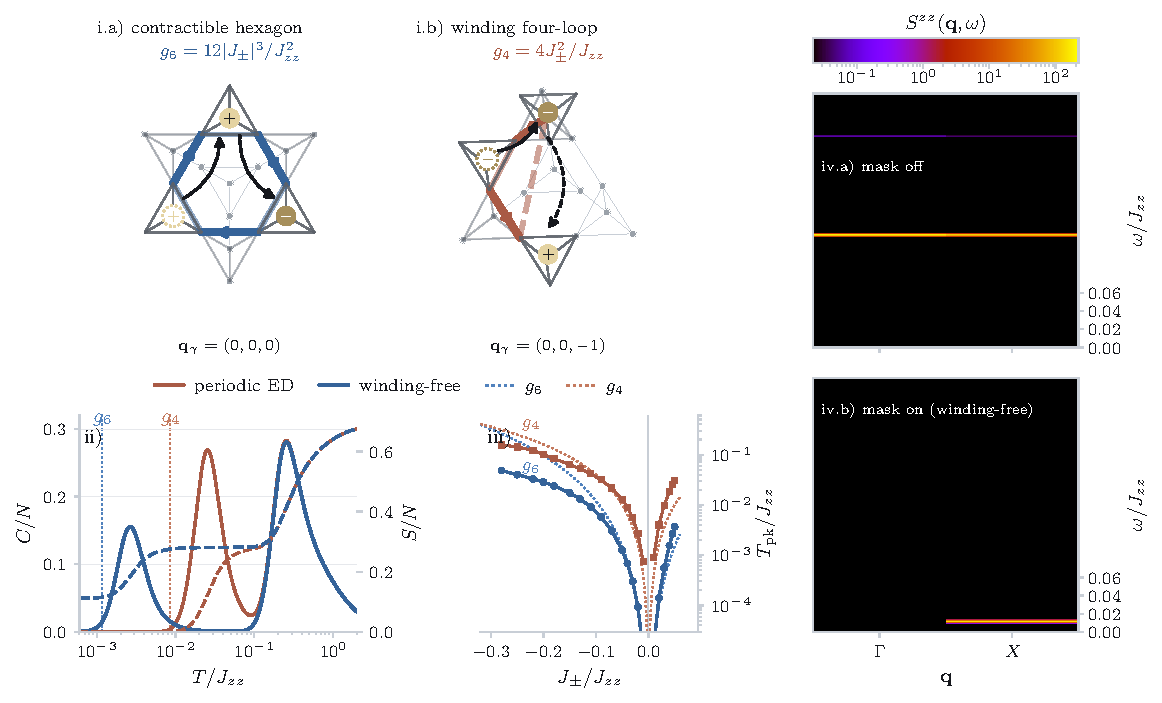
\includegraphics[width=\textwidth]{fig_summary.pdf}
\caption{Microscopic transport and winding removal on cubic-16.
(i.a),(i.b) The two shortest ice-to-ice processes on the 16-site torus. Gray
marks the cluster; colored circles and bonds are the loop, with its exchanges
numbered in order and each drawn as an arrow from the lowered to the raised
spin. An exchange leaves the tetrahedron it straddles neutral and charges the
two outer ones, so it creates, moves, or annihilates a spinon--antispinon
pair; charges sit at the centre of their tetrahedron, whose frame is drawn,
light for $Q_t>0$ and dark for $Q_t<0$, faded where a charge has since left.
The printed triple below each panel is the total transport $\bq_\gamma$ of
Eq.~(\ref{eq:transport}). (i.a) On the contractible hexagon the pair is
created, walks, and annihilates inside one cell: $\bq_\gamma=\bm0$, and the
process enters at third order, at the $g_6$ of Eq.~(\ref{eq:g6}). (i.b) The
winding four-loop closes only through the periodic identification (dashed
bond): it transports one unit of polarization across the cell,
$\bq_\gamma=(0,0,-1)$, enters already at second order, at the $g_4$ of
Eq.~(\ref{eq:g4}), and is removed by the mask of
Eq.~(\ref{eq:mask}), which retains the hexagon.
(ii),(iii) One color code and one legend serve both panels: periodic ED
(orange), the winding-free construction (blue), and the dotted perturbative
scales $g_6$ and $g_4$, labeled in each panel. (ii) Heat capacity (solid, left
axis) and entropy (dashed, right axis) at $(\Jpm,\Jpp)/\Jzz=(0.046,0)$,
each from the complete $65536$-level spectrum of the same cluster: the
periodic low-temperature peak sits at the artifact scale $g_4$, whereas the
winding-free peak moves down to the ring-exchange scale $g_6$. (iii) Position
of the low-temperature heat-capacity maximum across the coupling range: the
winding-free peak follows $g_6$ as $\Jpm\to0$ on both flux sides, while the
periodic peak tracks $g_4$ throughout.
(iv.a),(iv.b) Zero-temperature longitudinal structure factor
$S^{zz}(\bk,\omega)$ of the downfolded ice-block dynamics at a common anchor,
without and with the mask, on one logarithmic color scale, averaged over the
three symmetry-related $X$ points with broadening
$\eta=6\times10^{-4}\Jzz$. Because $S^z$ is diagonal in the Ising
configuration basis, $\Pice S^z_{\bk}\Pice$ is exactly a diagonal matrix and
both panels are the same $90\times90$ eigenvalue problem fed identical sources:
they differ only by whether Eq.~(\ref{eq:mask}) was applied, so the figure
isolates the artifact rather than the downfolding. No reference frame enters
either one.}
\label{fig:summary}
\end{figure*}

\emph{Introduction.}---Quantum spin ice (QSI) is a $U(1)$ quantum spin liquid
with fractionalized excitations and an emergent gauge field whose gapless
photon mode provides a characteristic low-energy signature
\cite{Hermele2004,Gingras2014,Benton2012}. Recent experiments on
Ce$_2$(Zr,Sn,Hf)$_2$O$_7$ suggest that Ce-based pyrochlores may realize a
$\pi$-flux QSI, in which an emergent gauge flux of $\pi$ threads each
elementary hexagonal plaquette [Fig.~\ref{fig:summary}(i.a)]
\cite{Gao2019,Gaudet2019,Bhardwaj2022}. In Ce$_2$Zr$_2$O$_7$, no long-range
order or spin freezing is observed down to the lowest accessible
temperatures. Its specific heat features one broad hump, whereas recent
heat-capacity measurements on Ce$_2$Hf$_2$O$_7$ resolve two anomalies near
$65\,$mK and $25\,$mK \cite{Smith2025}. Numerical linked-cluster fits on the
high-temperature tail of the specific heat measurement place the candidate
parameters within the $\pi$-flux QSI regime, which is a regime where the
average flux threaded through a plaquette is $\pi$. But a true microscopic
investigation of the origin of the two-peak structure is still lacking,
particularly on the low-temperature peak.

This is because obtaining a microscopic description of $\pi$-flux QSI using
unbiased numerical methods is challenging. Quantum Monte Carlo (QMC)
simulations access the zero-flux QSI \cite{Shannon2012,Kato2015,Huang2018} but
encounter a sign problem in the $\pi$-flux regime. Numerical linked-cluster
expansions fail to converge at the ultralow temperatures at which the lower
anomaly emerges. Finite-temperature tensor-network calculations have reached a
periodic 48-site three-dimensional Heisenberg cluster, but only well above the
ring-exchange scale \cite{Schaefer2020}. Density-matrix renormalization group
and minimally entangled typical thermal states reach lower temperatures on
pyrochlore tubes \cite{Hagymasi2021}, but their quasi-one-dimensional geometry
cannot support a gapless photon mode. A sign-unrestricted microscopic
treatment that resolves the three-dimensional gauge dynamics at temperatures
of order $g_6$ is therefore needed.

Exact diagonalization (ED) is precise on a finite cluster and imposes no sign
restriction, but is limited to small pyrochlore tori, notably the cubic
16-site and face-centered-cubic 32-site clusters. Their dominant artifact is
not size alone but the appearance of spurious four-site loops. To see this, we
first introduce the physics of the gauge sector dynamics. The minimal
microscopic setting for QSI is the nearest-neighbor pseudospin-$1/2$ XYZ model
\begin{equation}
\begin{aligned}
H_0={}&\Jzz\sum_{\langle ij\rangle}S_i^zS_j^z
-\Jpm\sum_{\langle ij\rangle}\left(S_i^+S_j^-+S_i^-S_j^+\right)\\
&+\Jpp\sum_{\langle ij\rangle}\left(S_i^+S_j^++S_i^-S_j^-\right),
\end{aligned}
\label{eq:model}
\end{equation}
with $\Jzz>0$. For $|\Jpm|,|\Jpp|\ll\Jzz$ the low-energy states obey the
spin-ice rule $Q_t\equiv\sum_{i\in t}S_i^z=0$ on every tetrahedron $t$; we
write $\Pice$ for the orthogonal projector onto that manifold, of rank $90$ on
cubic-16. Transverse exchange first connects distinct ice configurations at
third order, through collective flips around elementary six-site hexagons,
generating the ring-exchange scale [Fig.~\ref{fig:summary}(i.a)]
\begin{equation}
g_6=\frac{12|\Jpm|^3}{\Jzz^2}.
\label{eq:g6}
\end{equation}
In the convention of Eq.~(\ref{eq:model}), $\Jpm>0$ gives the zero-flux QSI,
whereas $\Jpm<0$ gives the $\pi$-flux QSI. The parametrically small scale
$g_6$ is therefore a natural candidate for the lower-temperature
thermodynamic anomaly.

On cubic-16, a noncontractible four-spin path closes through the periodic
boundary [Fig.~\ref{fig:summary}(i.b)] and contributes already at second
order, with
\begin{equation}
g_4=\frac{4\Jpm^2}{\Jzz},
\qquad
\frac{g_4}{g_6}=\frac{\Jzz}{3|\Jpm|},
\label{eq:g4}
\end{equation}
whereas the physical hexagon process appears only at third order. The artifact
therefore diverges relative to the physical process in exactly the
perturbative limit where the cluster would otherwise be most trustworthy.
Cubic-16 hosts 36 such winding four-cycles against 16 contractible hexagons;
FCC-32 reduces but does not remove the problem, with 24 winding four-cycles,
32 contractible hexagons, and 96 wrapping hexagons. Due to the poor scaling of
ED we cannot reach a cluster on which the four-site loop is absent.

In this Letter we remove the artifact by coupling microscopic spin transfers
to an auxiliary source that records their net transport on the covering
lattice---the infinite lattice obtained by unwrapping the periodic cell into
translated copies---and retaining only the zero-transport component. Our first
methodological result is that this projection needs neither a reference frame
nor a spectrally isolated band: it is realized exactly by the Feshbach map
onto the combinatorial ice manifold, and as a genuine Hermitian operator by a
counterterm supported inside that manifold. Our central result concerns the
one apparent blemish of that operator, the energy at which the counterterm is
exact. We show that this energy is fixed by a self-consistency condition, that
at its solution the construction is exact for the ground multiplet including
the degeneracy which the transport-sector decomposition forces, and that
solving the condition to high precision---rather than iterating it a few
times---removes what we had previously mistaken for an intrinsic residue. We
close by measuring what actually limits the whole family of constructions.

\emph{Transport character.}---Periodic boundary conditions identify virtual
processes that remain distinct on the covering lattice. In the elementary
hexagonal process an $S^+S^-$ operation creates a spinon--antispinon pair,
which propagates around a contractible hexagon and annihilates. The spurious
four-site process closes only through the periodic identification: on the
covering lattice it is not a closed loop but an open string that transports one
defect across a period before the pair recombines. Both connect ice states and
have identical endpoints on the torus; their topology differs only on the
cover.

A periodic cluster is specified by three period vectors, collected as the rows
of a $3\times3$ matrix $L$, and site positions $\br_i$ in a chosen fundamental
cell. For every oriented bond $(i,j)$ we choose $\bn_{ij}\in\mathbb Z^3$ such
that the covering-lattice image of $j$ connected to $i$ is
$\bm R_{j|i}=\br_j-\bn_{ij}^{T}L$, so $\bn_{ij}=0$ for an intracell bond. For a
configuration $\mathcal C$ lifted continuously to the cover we introduce the
polarization coordinate
\begin{equation}
\bm p(\mathcal C)=\sum_{i=1}^{N} S_i^z(\mathcal C)\,\bm R_i ,
\label{eq:polarization}
\end{equation}
the first spatial moment of the site-resolved Ising polarization. It
introduces no physical degree of freedom and is not a dipole moment; its only
role is to record how $S^z$ is displaced by a sequence of microscopic
operations. For any sequence $\gamma$ the accumulated transport is
\begin{equation}
\bq_\gamma=2\sum_{\ell\in\gamma}\Delta\bm p_\ell .
\label{eq:transport}
\end{equation}
The factor of two is a quantization requirement rather than a convention.
With $S^z=\pm\tfrac12$ the raw increments are half-integer multiples of the
periods, and doubling promotes every closed ice-to-ice sequence to an integer
vector in units of the cluster periods, as in $\bq_\gamma=(0,0,-1)$ of
Fig.~\ref{fig:summary}(i.b). Integrality is what makes
$e^{-i\btheta\cdot\bq_\gamma}$ a character of the source torus, and hence the
average over $\btheta$ a genuine group-orthogonality sum,
$(2\pi)^{-3}\int d^3\btheta\,e^{-i\btheta\cdot\bq_\gamma}
=\delta_{\bq_\gamma,\bm0}$. A half-integer label would be \emph{mutilated} by
the same average rather than removed---a point we return to, because it is
what ultimately bounds the method.

Since $\bq$ is conserved by every physical ice-to-ice process, the
winding-free effective Hamiltonian on the ice manifold is block diagonal in
the transport sectors, and the projection is implemented by the mask
\begin{equation}
\bigl(\Delta[A]\bigr)_{ab}=A_{ab}\,\delta_{\bq_a,\bq_b},
\label{eq:mask}
\end{equation}
which deletes exactly the boundary-winding matrix elements. On cubic-16 the
$90$ ice configurations fall into $25$ such sectors, of dimensions
\begin{equation}
6\times1+12\times2+6\times8+1\times12=90 .
\label{eq:sectors}
\end{equation}
Sectors related by a cubic operation carry identical spectra under any masked
operator. The winding-free spectrum therefore has \emph{exact} degeneracies,
and Eq.~(\ref{eq:sectors}) is what fixes them; this is used below.

\emph{Frame-free downfolding.}---The construction requires an effective
Hamiltonian on the ice manifold to which Eq.~(\ref{eq:mask}) can be applied.
Previous implementations obtained one by projecting the exact low-energy band
onto $\Pice$ and orthonormalizing with the canonical polar isometry. That
route requires the band to remain spectrally isolated and the projected Gram
matrix $\Pice P\Pice$ to remain invertible, and we show below that both fail
well before the couplings of experimental interest.

Neither is necessary. Splitting the Hilbert space with $P=\Pice$ and
$Q=1-P$ and eliminating $Q$ exactly gives the Feshbach map
\begin{equation}
F(z)=PH_0P+PH_0Q\,(z-QH_0Q)^{-1}QH_0P ,
\label{eq:feshbach}
\end{equation}
whose self-consistent roots $E=\mathrm{eig}\,F(E)$ are exact eigenvalues of
$H_0$ with nonzero ice weight. Nothing here refers to eigenvectors, to
adiabatic continuation, or to a Gram matrix: $P$ is combinatorial and exists at
every coupling. Each sorted branch of $F$ is monotone between poles of the
self-energy, so every root below the continuum is located by guaranteed
bisection; against the exact spectrum at $\Jpm/\Jzz=-0.05$ the ninety unmasked
roots reproduce the lowest ninety eigenvalues to $3\times10^{-13}\Jzz$. The
mask of Eq.~(\ref{eq:mask}) is a pinching and preserves that monotonicity, so
$\Delta[F(z)]$ inherits the same guarantee. We take the masked roots as the
\emph{reference} winding-free spectrum throughout.

\emph{The counterterm.}---The masked map delivers the gauge sector but not the
rest of the Hilbert space: it has no states above the band, so it yields
neither the spinon anomaly nor any observable requiring a wavefunction. For
those one needs an operator. Let $C=C^\dagger$ be supported inside the ice
manifold, $C=PCP$. Then $Q(H_0+C)Q=QH_0Q$ and $Q(H_0+C)P=QH_0P$: the
self-energy is untouched, and
\begin{equation}
F_{H_0+C}(z)=F_{H_0}(z)+C
\qquad\text{for every }z .
\label{eq:ct}
\end{equation}
A counterterm living inside $P$ has no matrix element reaching the spinon
sector and therefore cannot dress itself; it enters the effective theory with
exactly the coefficient chosen. Choosing
\begin{equation}
C=-\bigl(1-\Delta\bigr)\bigl[F_{H_0}(z_0)\bigr]
\label{eq:Cchoice}
\end{equation}
makes $F_{H_0+C}(z_0)=\Delta[F_{H_0}(z_0)]$ exactly: the winding-free effective
Hamiltonian is realized as the Feshbach map of a genuine Hermitian operator on
the full Hilbert space. Every transporting process---four-cycles, wrapping
hexagons and the longer transporting strings---is cancelled at once, with no
loop-class enumeration and no perturbative hierarchy, at a cost of ninety
linear solves per evaluation.

\emph{The anchor is not a parameter.}---Equation~(\ref{eq:Cchoice}) is exact at
$z_0$ and approximate elsewhere, and this is the only respect in which the
operator falls short of the map. The resolution is that $z_0$ is not free. It
is determined by the Brillouin--Wigner condition
\begin{equation}
z_0=E_0\bigl(H_0+C(z_0)\bigr) ,
\label{eq:bw}
\end{equation}
and at a solution of Eq.~(\ref{eq:bw}) the ground state of $H_0+C$ sits exactly
at the one energy where the counterterm is exact. The winding-free ground
multiplet is therefore reproduced not approximately but exactly---and in
particular with the degeneracy that Eq.~(\ref{eq:sectors}) forces, which is a
theorem about the mask rather than a numerical coincidence. We verify that the
protected degeneracies of $\Delta[F(z_0)]$ hold to $6\times10^{-7}$ of the band
width at every coupling, and that the multiplicity is $6$ throughout
$\Jpm/\Jzz\ge-0.22$, changing to $2$ from $-0.25$ on as the sector structure
reorganizes.

Everything then depends on how well Eq.~(\ref{eq:bw}) is solved, and this is
the point we had previously missed. Iterating $z\mapsto E_0(H_0+C(z))$
converges linearly at rate $\sim1-Z$, where $Z$ is the ice weight introduced
below; at $\Jpm/\Jzz=-0.20$, where $Z\simeq0.5$, that is a factor of two per
expensive solve. A secant step on $g(z)=E_0(H_0+C(z))-z$ costs the same and
converges superlinearly, reaching $|g|<10^{-13}$ in five to eleven
solves. Tracking the
splitting $\delta$ of the protected ground multiplet along that trajectory
gives, at $\Jpm/\Jzz=-0.20$,
\begin{equation}
\delta\simeq1.5\,|g|
\label{eq:proportional}
\end{equation}
over ten decades, from $\delta=4\times10^{-2}$ at $|g|=6\times10^{-2}$ down to
$\delta=1\times10^{-12}$ at $|g|=5\times10^{-15}$ \cite{SM}.

The consequence is a correction to our own earlier reading of this
construction. An under-converged anchor splits the protected multiplet; by the
Schottky relation a splitting $\delta$ manufactures a heat-capacity anomaly at
$T\approx\delta/2.4$, and it simultaneously breaks the entropy sum rule
$\int_0^\infty(C/NT)\,dT=N^{-1}\ln(2^N/g_0)$, because levels split too finely
to release entropy are also not exactly degenerate enough to count as frozen.
Both effects are real and we had reported them---a spurious low-temperature
peak at every coupling, and a $10\%$ sum-rule violation at weak coupling---as
an intrinsic ``anchoring residue'' requiring a repair. Equation
(\ref{eq:proportional}) shows they are neither intrinsic nor in need of repair:
with Eq.~(\ref{eq:bw}) solved to $10^{-13}$ the worst splitting anywhere in
the sweep is $\sim10^{-12}\Jzz$, the anomaly it could produce lies twelve
orders of magnitude below $g_6$, the sum rule is satisfied to
$5\times10^{-7}$ at every coupling with the measured $g_0$, and no maximum of
$C(T)$ appears at the residual scale.

A third maximum does appear, but for a different and physical reason, and only
for $|\Jpm|/\Jzz\ge0.22$. The protected multiplet is separated from the rest
of the band by a genuine gap, which produces its own Schottky anomaly; at weak
coupling that anomaly coincides with the ring anomaly and at strong coupling it
resolves from it. It is present in the exact masked reference, whose gap the
counterterm reproduces to $3\%$, so it is a property of cubic-16's
twenty-five-block structure rather than of the method. This is precisely what
the unconverged variant obscured: it produced a spurious branch at
\emph{every} coupling, including those where the physical one is merged.

We also tested the repair we had proposed, and it makes things worse. The
degeneracy pattern of $\Delta[F(z_0)]$ is exact, so one can read the protected
multiplets off it and average the counterterm spectrum within each; averaging
is the unique trace-preserving choice. Applied to the converged spectrum this
degrades the ring-exchange scale from $0.66\%$ to $1.16\%$ of the reference at
$\Jpm/\Jzz=-0.20$, and from $1.86\%$ to $2.65\%$ at $-0.22$. The reason identifies where the counterterm's real error
lives: Eq.~(\ref{eq:Cchoice}) is exact at $z_0$, so $\Delta[F(z_0)]$ describes
the bottom of the band well and the top badly---by mid-band at $-0.20$ its
levels overshoot the reference by more than a factor of two---and while its
degeneracy pattern is exact its eigenvectors are not, with an overlap purity of
only $0.57$. The counterterm's residual error is the ordinary $O(1-Z)$ energy
dependence of the exact downfolded theory spread through the upper band, and
the correct response is to place the exact point where the physics is decided
and then quote $Z$, not to post-process the spectrum.

\begin{figure}[t]
\centering
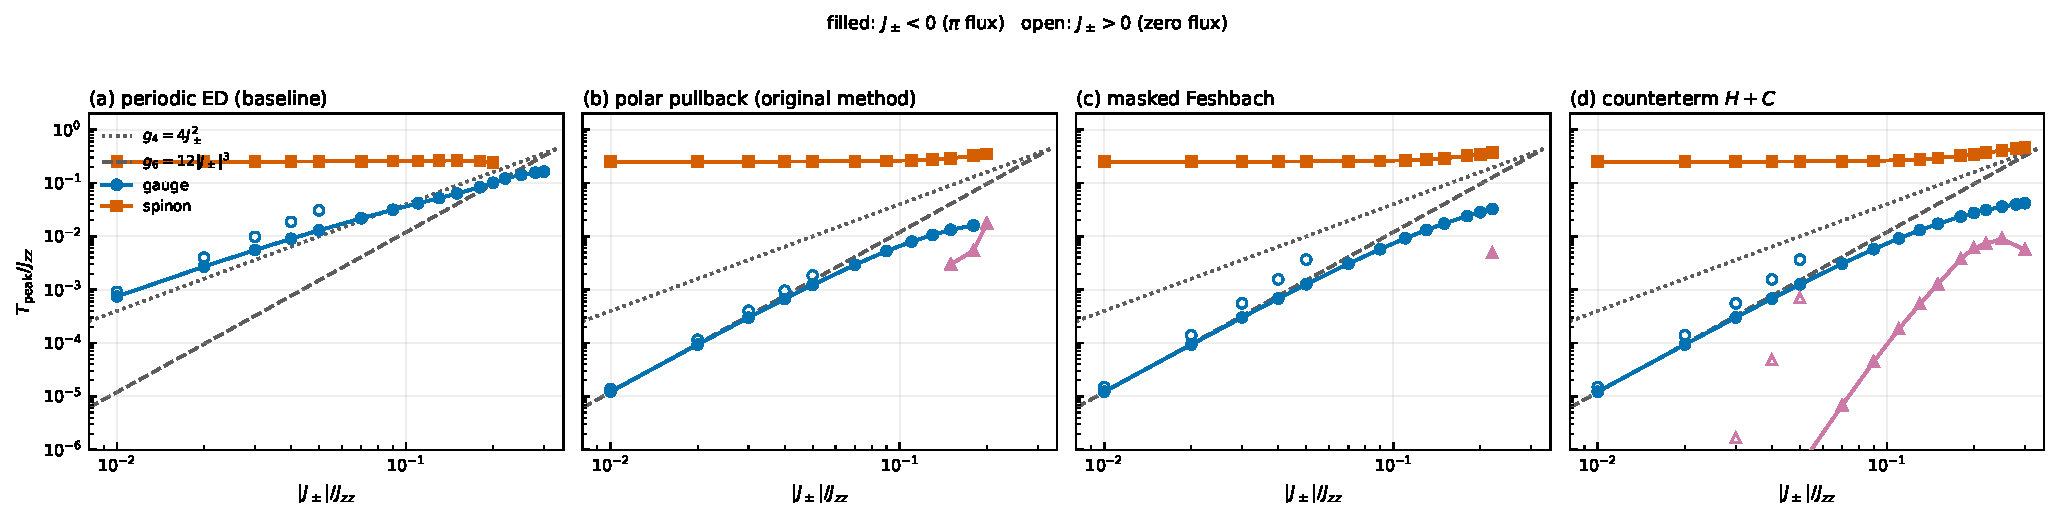
\includegraphics[width=\linewidth]{fig_peak_tracking.pdf}
\caption{Every maximum of $C(T)$ tracked across coupling against the two
candidate scales: the baseline, and the counterterm before and after the anchor
is converged. Circles: the ring (for periodic ED, gauge) anomaly. Triangles:
transport-sector anomalies. Squares: the spinon anomaly. Filled symbols are the
$\pi$-flux side, open the zero-flux side. Periodic ED tracks $g_4$ throughout;
the winding-free construction tracks $g_6$. Panel (b) is the counterterm with the anchor
iterated three times, as in an earlier version of this work: a sector branch
runs along the bottom at every coupling. Panel (c) is the same construction
with Eq.~(\ref{eq:bw}) solved to $10^{-13}$: that branch is gone, and the
sector anomaly that remains for $|\Jpm|/\Jzz\ge0.22$ is the physical
multiplet gap, present in the exact reference too.}
\label{fig:tracking}
\end{figure}

\emph{Results.}---We computed the complete $65536$-level spectrum---every
magnetization sector, translation resolved---at $22$ couplings spanning
$-0.30\le\Jpm/\Jzz\le0.05$, and evaluated $C(T)$ from each. The counterterm
modifies only the $S^z_{\rm tot}=0$ block, so the remaining sectors are shared
with periodic ED exactly. Every peak is labelled by the number of thermally
active levels that produce it; the checks (anchor residual, protected
degeneracies, entropy sum rule, temperature-grid refinement, mask convergence)
are reported in the Supplemental Material \cite{SM}.

The separation of scales is unambiguous (Fig.~\ref{fig:tracking}). The
winding-free anomaly settles onto the ring-exchange scale as $\Jpm\to0$, as it
must since perturbation theory becomes exact there: $1.024\,g_6$ at
$\Jpm/\Jzz=-0.01$ and $1.245\,g_6$ at $+0.01$. Neither is exactly $g_6$, nor
should it be---a Schottky maximum sits at $\Delta/2.4$ only for a two-level
system, and the prefactor depends on how the ninety band levels are
distributed, which differs between the frustrated and unfrustrated signs.
Ordinary periodic ED instead approaches $1.87\,g_4$ and departs from $g_6$ as
$g_4/g_6\propto1/|\Jpm|$, by a factor $62$ at $\Jpm/\Jzz=-0.01$. Fitting
$T_{\rm peak}\propto|\Jpm|^{n}$ over $|\Jpm|\le0.03$, with peak positions
refined below the temperature-grid spacing, gives $n=1.99$ for periodic ED
against the ideal $2$ of $g_4$, and $n=3.10$ for the winding-free construction
against the ideal $3$ of $g_6$.

Two comparisons with the frame-free reference are worth separating. The
sharpest is the ground energy, where the fixed point makes a parameter-free
prediction: it agrees with the lowest exact masked root to between
$10^{-15}$ and $7\times10^{-13}\Jzz$ at every coupling. The ring anomaly agrees
to $0.18\%$ or better throughout $|\Jpm|/\Jzz\le0.18$, degrading to $0.66\%$ at
$-0.20$ and $1.86\%$ at $-0.22$. Individual band \emph{levels} are far less
accurate than either: the largest deviation grows from $0.12\%$ of the band
width at $-0.01$ to $16.3\%$ at $-0.20$. That hierarchy---an exact ground
energy, a per-cent-accurate anomaly, and levels an order of magnitude
worse---is the signature of a construction exact at one energy and degrading
away from it, and the anomaly survives it because its position is set by how
the band is distributed rather than by where any individual level sits.
Beyond $-0.22$ the reference loses branches; they are not missing states but
real-energy bound states in the continuum, protected by transport
superselection, that the root finder cannot reach \cite{SM}. The spinon anomaly
is essentially common to both constructions at weak coupling
($0.25307\,\Jzz$ against $0.25282$ for periodic ED at $-0.05$), as it should be
since neither modifies the spinon sector; it separates at strong coupling
($0.347$ against $0.241$ at $-0.20$) not because that sector changed but
because removing the $g_4$ network compresses the gauge band underneath it, and
the position of a maximum depends on the whole spectrum.

One prediction of the construction is worth isolating, because it is
qualitative and requires no reference. The transport label of
Eq.~(\ref{eq:transport}) is a linear function of the four sublattice
magnetizations, so on cubic-16 the $\bk=0$ operator $\Pice S^z_{\bm0}\Pice$ is
\emph{exactly} constant within each transport sector---one value per sector, to
machine precision. It therefore commutes with the mask and is a function of the
conserved label, and cannot connect the winding-free ground multiplet to
anything: the winding-free longitudinal response at $\bk=0$ vanishes
identically, measured as $5\times10^{-30}$ against $0.333$ for the same
quantity with the mask removed. The entire $\bk=0$ longitudinal weight that
ordinary periodic exact diagonalization reports on this cluster is boundary
artifact.

At the sign-free benchmark $(\Jpm,\Jpp)/\Jzz=(0.046,0)$ the winding-free
maximum lies at $2.27\,g_6$ against $0.94\,g_6$ from QMC in the thermodynamic
limit \cite{Huang2018}, while ordinary ED gives $22\,g_6$: the construction
agrees with QMC on the \emph{scale} but differs by a factor of two, as does the
polar pullback in the other direction ($1.24\,g_6$). That spread is not a test
of the method---the same peak moves by a factor of three between cubic-16 and
FCC-32, so a $16$-site cluster cannot resolve a factor of two against the
thermodynamic limit \cite{SM}. The sharp validations are internal: the exact
ground energy, the $0.2\%$ ring agreement, and the $g_6$ exponent.

\emph{What limits the method.}---All constructions degrade, and they do so for
one shared reason. The Supplemental Material \cite{SM} collects every failure
metric beside the residue $Z=[1-\langle\partial_z\Sigma\rangle]^{-1}$, the
fraction of the true eigenstate carried by the ice manifold. The Gram minimum
of the polar route \emph{is} $Z$ to within a few per cent; the disagreement
between constructions is $0.4(1-Z)/Z$; root loss in the reference begins at
$Z\approx0.37$. Across the range studied $Z$ falls from $0.99$ to $0.26$,
because virtual spinon pairs proliferate as
$\langle n_{\rm pairs}\rangle\approx2N(\Jpm/\Jzz)^2$.

The conflict is structural. The mask requires an integer transport label, and
the label is an integer only on the ice manifold, since a single spinon hop
displaces $\bm p$ by a quarter period and would be mutilated rather than
removed by the character average. The model space is therefore forced to be
the ice manifold, while describing the physics at large $|\Jpm|$ requires
precisely the spinon admixture the mask cannot accommodate. One cannot enlarge
the model space to improve $Z$ without destroying the label the construction
rests on.

What does \emph{not} happen is worth stating, since we had previously suspected
otherwise. Nothing singular occurs to the cluster: the ground state stays
nondegenerate, the gap grows monotonically, and every dressing measure is
smooth---in particular there is no feature at $\Jpm/\Jzz=-0.23$, where an
earlier reading of a coherence diagnostic had placed a boundary. The $\pi$-flux
side does not go transverse-ordered, and the winding-free gauge sector does not
stop existing: read off the exact map it remains a ring-exchange model with
negligible potential ($|V/g|\le0.012$, excluding a Rokhsar--Kivelson freezing
scenario) whose amplitude grows in absolute terms while becoming progressively
longer ranged \cite{SM}. The spinon sector retains its own finite-size error,
which we measure by twisting the boundary condition: the spinon threshold moves
by $3.8\%$ of its gap at $-0.05$ and $24.8\%$ at $-0.30$, against an
ice-sector response of several times $g_4$---an ordinary finite-size effect, not
a second copy of the winding artifact, because a spinon path around the box has
a bulk counterpart at the same order whereas the winding four-cycle has none.

\emph{Outlook.}---The self-consistent counterterm is, on the evidence assembled
here, the construction to use: it needs no reference frame, no isolated band and
no fitted correction, satisfies the entropy sum rule identically, reproduces the
exact masked ground energy to machine precision and the ring anomaly to
$0.2\%$, produces both thermodynamic anomalies and all observables from a
single diagonalization, and continues past the coupling at which the reference
loses branches. Its remaining limitations are quantified rather than hidden: an
$O(1-Z)$ error in the upper band, an untouched spinon sector, and a cluster
whose winding-free blocks are at most twelve-dimensional---narrow enough that
by $\Jpm/\Jzz=-0.30$ the band has grown as wide as the spinon scale and the
ring anomaly ceases to be a separate maximum at all. The last of these is the one that
matters most. Comparing cubic-16 with FCC-32 at matched truncation moves the
ring anomaly by a factor of $2.4$ to $3.5$---larger than every other
uncertainty in the calculation combined. On FCC-32 the transport sectors reach
dimension $396$ and the construction applies unchanged; that is where the
quantitative photon thermodynamics of the $\pi$-flux candidates should be
computed.

\begin{acknowledgments}
\end{acknowledgments}

\bibliography{references}

\end{document}
